\section{Theorie}
\subsection{Radioaktiver Zerfall}
Der beim radioaktiven Zerfall verwandelt sich ein instabiler Kern in einen leichteren unter Emission von Teilchen. Es existieren mehrere Arten von radioaktiven Zerfall: 
\begin{itemize}
 \item $\alpha$\\
  {Bei dieser Zerfallsart stößt der Kern einen Heliumkern (ohne Elektronen) aus. Die Veränderung folgt diesem Schema:
  $$_Z^AX \rightarrow _{Z-4}^{A-2}Y + _4^2He^{2+}$$}
 \item $\beta^-$\\
 {Bei dieser Zerfallsart zerfällt ein Neutron in ein Proton unter der Emission von einem Elektron und einem Antielektroneutrino.  
 $$n\rightarrow p+e^-+\bar{v}_e$$} 
 \item $\beta^+$\\
 {Bei dieser Zerfallsart zerfällt ein Proton in ein Neutron unter Emission von eines Positrons und Elektroneutrinos.
 $$p\rightarrow n+e^++v_e$$}
 \item Electron Capture\\
  {Dieser Zerfall ist ähnlich zum $\beta^+$ Zerfall, da auch ein Neutron in ein Proton umgewandelt wird. Der unterschied hier ist, dass ein Elektron eingefangen wird.
 $$n\rightarrow p+e^-+\bar{v}_e$$}
\end{itemize}

\subsection{$\gamma$ Strahlung}
Die Zerfällt ein Kern über die oben genannten Zerfälle, hat der Tochterkern oft noch eine Restenergie, da es zufällig ist welche Energie nach dem Zerfall entstehen. Die angeregten Tochterkerne geben diese überschüssige Energie in Form von $\gamma$ Photonen ab. Die Energien der $\gamma$ Photonen liegen Zwischen keV bis MeV. 
\subsubsection{Wechselwirkungen von Materie mit $\gamma$ Photonen}
Die Interaktion von $\gamma$ Photonen ist Abhängig von der Masse des Interagierenden Kerns und der Energie des $\gamma$ Photon.
\begin{itemize}
	\item Photoelektrischer Effekt\\
	Hierbei wird das $\gamma$ Photon direkt von einem Elektron absorbiert. Die Energie des Photons wird komplett in kinetische Energie umgewandelt. Die so entstandene Lücke wird mit Elektronen aus höheren Schalen unter Abstrahlung von Röntgenstrahlung und Augerelektronen gefüllt. Dieser Effekt findet meist bei einer Energie $E_\gamma<200\,$keV und einer Atommasse von 50 statt.

	\item Compton Streuung\\
	Im Unterschied zum Photoelektrischen Effekt werden die $\gamma$ Photonen nicht absorbiert sondern streuen an den Elektronen. Hierbei geben sie einen Teil ihrer Energie ab.
	Compton Streuung findet meist bei einer einergie von $200\,$keV$<E_\gamma<5\,$MeV statt. Die Atommassen sind ähnlich zu denen des Photoeffekts.
	
	\item Paarbildung\\
	Wenn die Energie $E_\gamma$ eine kritische Energie von $1.022\,$MeV überschreitet, kann Paarbildung auftreten. Wenn ein $\gamma$ Quant in das elektromagnetische Feld eines Elektrons oder Atomkerns kommt, kann es sich in ein Elektron-Positron Paar aufspalten. 
		$$\gamma \rightarrow e^- + e^+$$
	Dies erklärt auch die kritische Energie von $1.022\,$MeV, was die doppelte Ruhemasse eines Elektrons ist. Energie des $\gamma$ Photons über dieser Schwelle wird als Kinetische Energie der entstanden Teilchen  weitergegeben. 
	Das entstandene Positron ist sehr kurzlebig und zerstrahlt kurz nach entstehen mit einem Elektron in zwei $\gamma$ Photonen mit einer Energie von jeweils $511\,$keV unter einem Winkel von $180^\circ$ zu einander. 
\end{itemize}

\subsection{Nachweis von $\gamma$ Photonen}
Die hochenergetischen Photonen werden mittels eines Szintillators nachgewiesen. Dies sind Materialien, welche die $\gamma$ Photonen absorbieren und in Photonen kleinerer Energien aufspalten. Diese werden mittels eines Photomultipliers Detektiert. 
Im allgemeinen unterscheidet man zwischen zwei Verschiedenen Szintillator Typen.
\subsubsection{Anorganischer Szintillator}
Der in diesem Versuch verwendete anorganische Szintillator besitzt einen Natriumiodid Kristall, welcher mit Thallium dotiert ist.
Die vom Kristall absorbierten $\gamma$ Photonen besitzen die Energie, hunderte bis tausende Elektonen vom Valenz- ins Leitungsband  zu bewegen. An Stelle der Elektronen bleiben Löcher zurück. 
Nach einiger Zeit verlieren die angeregten Elektronen im Leitungsband ihre Energie unter Abstrahlung eines Photons. Ohne Dotierung würden die so emittierten Photonen wieder absorbiert werden  und der Kristall wäre für diese undurchsichtig. 
Durch die Dotierung werden Aktivator Zentren erzeugt, an welchen der Übergang zwischen Valenz- und Leitungsband weniger Energie benötigt. Dies ist in Abbildung \ref{bänder_NaJ} zu sehen.  An diesen Aktivator Zentren rekombinieren die Elektron-Loch Paare unter Abgabe von Photonen auf Aktivator Niveau. Diese Photonen werden von der Mehrheit des Kristalls nicht Absorbiert und können vom Photomultiplier detektiert werden.\\

\begin{figure}
	\centering
	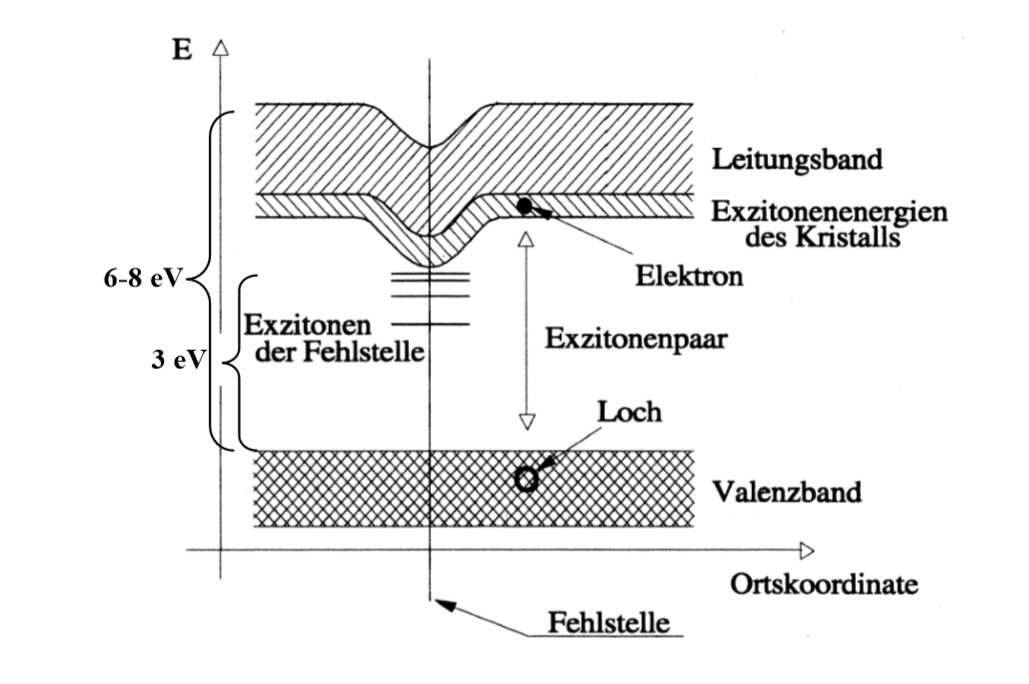
\includegraphics[scale=0.7]{Bilder/baendermodell}
	\caption[Bändermodell in dotiertem NaJ]{\small Bändermodell des Natriumiodid Szintillators, der mit Thallium dotiert ist. Entnommen aus \cite{staatsex_szinti}}
	\label{bänder_NaJ}
\end{figure}
Die hohen Atomaren Massen der Gitteratome des Kristalls ermöglichen eine gute Absorption der $\gamma$ Photonen. Das führt zu einer hohen Lichtausbeute und geringen statistischen Schwankungen. Deshalb ist der Natriumiodid Szintillator gut für Energiemessungen geeignet. Die An- und Abregung des Kristalls findet aber auf einer Zeitskala von $100\,\mu$s statt, was die Zeitauflösung dieses Szintillators beschränkt. 

\subsubsection{Organischer Szintillator}
Der im Versuch verwendete Plastikszintillator gehört zur Gruppe der Organischen Szintillatoren. Hier erzeugen die $\gamma$ Photonen geladene Teilchen, welche wiederum die Moleküle des Plastiks anregen. Diese übertragen die Energie auf Moleküle der Aktivtorsubstanz. Analog zum Anorganischen Szintillator haben diese auch eine unterschiedliche Energiedifferenz zwischen Angeregtem- und Grundzustand als die Moleküle des Plastiks.
Die Photonen der Aktivtorsubstanz können deshalb Detektiert werden.\\

Die Abklingzeit des Plastiks beträgt $8\cdot 10_{-9}\,$s, was in einer guten Zeitauflösung resultiert. Durch die niedrigeren Atommassen der Atome im Plastik ist eine Absorption der $\gamma$ Photonen unwahrscheinlicher. Dies resultiert in einer schlechteren Energieauflösung.

\subsubsection{Photomultiplier}
Der Aufbau eines Photomultipliers ist in Abbildung \ref{photomul} zu sehen. 

\begin{figure}
\centering
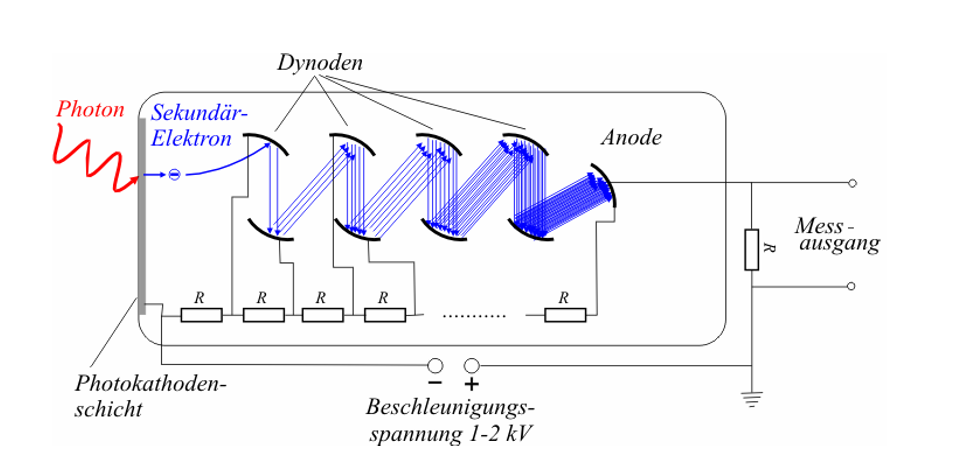
\includegraphics[scale=0.7]{Bilder/photomul}
\caption[Aufbau Photomultiplier]{\small Schematischer Aufbau eines Photomultipliers. Entnommen aus \cite{staatsex_szinti}}
\label{photomul}
\end{figure}

Die Photonen aus beiden Szintillatoren werden durch einen Photomultiplier detektiert. Eintreffende Photonen schlagen mittels des Photoeffektes Elektronen aus der Photokathode aus. Die Elektronen werden anschließend zu ersten Dynode mittels eines Elektrischen Feldes transportiert. Hier werden Sekundärelektronen ausgeschlagen. Diese werden anschließend vom Elektrischen Feld der nächsten Dynode angezogen, was zu einer kaskadierten Ladungsvervielfältigung führt. 

\section{Signalverarbeitung}

\subsubsection{Photomultiplier und Vorverstärker}
Im Szintillatormaterial wird ein Einfallendes $\gamma$ Photon in mehrere Photonen mit niedrigerer Energie umgewandelt. Diese entstehen kurz nach einander.
Die Photonen werden im Photomultiplier detektiert und als Stromsignal ausgegeben. \\
Der Vorverstärker ist in diesem Versuch direkt in die Betriebseinheit des Photomultipliers eingebaut. Dies verkürzt die Signalleitungen und damit die Störanfälligkeit des Ladungssignals aus dem Photomultipliers. In diesem werden auch mehrere der Ladungsimpulse des Photomultipliers durch ein RC-Glied integriert und in leichter zu übertragende Spannungspulse umgewandelt. Diese werden anschließend durch den Hauptverstärker weiterverarbeitet.

\subsection{NIM-Module}
NIM (Nuclear Instrument Module) ist ein Standard für Messeinstromente der Nuklearphysik. Es ist ein Modulares System, bei welchem die einzelnen Messgeräte eine standardisierte Größe besitzen und an der Rückseite Standardisierte Anschlüsse zur Energieversorgung besitzen. Alle in diesem Versuch verwendete Signalverarbeitungselektronik außer dem Vorverstärker, Oszilloskop und PC besitzt diesen Standard. 
\subsubsection{Hauptverstärker}
Der Hauptverstärker Verstärkt die schwachen Signale des Vorverstärkers in Signale mit größerer Amplitude. Die Verstärkung ist grob und fein Einstellbar. Außerdem ist die Shaping-Time konfigurierbar, also die Zeit in welcher die Signale zur weiteren Verarbeitung geformt werden. Es ist darauf zu achten, dass die Shaping-Time die Anstiegszeit des zu verstärkenden Signals nicht unterschreitet sodass die Energieinformationen des Signals nicht verloren gehen. Aber die Shaping-Time sollte so kurz wie möglich gewählt werden, sodass die Totzeit des Detektors minimiert ist. \\
Die Amplitude der Signale des Hauptverstärkers ist Proportional zur Energie der Detektierten Teilchen.
\subsubsection{Multichannel Analyzer (MCA)}
Der MCA Sortiert die eingehenden Signale anhand ihrer Amplitude in verschiedene Kanäle ein und speichert diese bzw. sendet sie an den PC. Die Amplitude der Signale variiert zwischen den Verschiedenen Versuchsaufbauten, sodass eine Kalibriermessung an einem bekannten Isotop durchgeführt werden muss, um den aktuellen Zusammenhang zwischen Detektor Kanal und Energie zu bestimmen.
\subsubsection{Singlechannel Analyzer (SCA)}
Der SCA dient zur Signaldiskriminierung. Es ist ein Fenster Einstellbar, sodass alle Signale höherer oder niedrigerer Amplitude als eingestellt ignoriert werden. 
\subsubsection{Koinzidenz Einheit}
Die Koinzidenzeinheit vergleicht zwei eingehende negative Rechtecksignale, ob diese Zeitgleich vorliegen. Ist dies der Fall wird ein negatives Rechtecksignal ausgegeben.
\subsubsection{Timing Unit}
Die Timing Unit modifiziert ein eingehendes negatives Rechtecksignal. Es ist möglich, die Dauer des Signals anzupassen und die Polarität umzukehren.
\subsubsection{Gate Generator}
Bei einem eingehenden Signal am Gate Generator leitet dieser für eine gewisse Zeit, Signale weiter. Sonst blockiert er die Signale.
\subsubsection{HEX-Counter}
Der HEX-Counter ist ein Zählgerät, welches für einen gewissen, einstellbaren Zeitraum die eingehenden negativen Impulse zählt.


\subsection{Oszilloskop}
Das Oszilloskop zeichnet Spannungssignale gegenüber der Zeit auf. Es kann diese Signale auch dauerhaft speichern. Es ist darauf zu achten, die Impedanz des Oszilloskops an die der NIM-Module anzupassen, da die Eingangsimpedanz des Oszilloskops $1\,\textrm{M}\Omega$ beträgt. Dies kann durch eine Reihenschaltung von Oszilloskop und $50\,\Omega$ Widerstand erreicht werden.

\subsection{PC}
Der PC kann die Daten des MCA auslesen und zur Weiterverarbeitung abspeichern. Hierzu stehen mehrere Dateiformate zur Verfügung. Bei einer Auswertung in Python ist das *.TKA Format empfohlen. 

\section{Verwendete Isotope}
Während des Versuches wurden die Nachfolgenden Isotope verwendet. Es werden nur die erwarteten deutlich Messbaren Zerfälle gelistet.
\subsection{Natrium}
Das ($^{22}Na$) Isotop von Natrium zerfällt am häufigsten mittels $\beta^+$  Zerfall in den Angeregten Zustand von $^{22}Ne$. Die überschüssige Energie des Neon Kerns wird in Form eines $\gamma$ Photons der Energie 1275 keV Abgegeben. Da diese Photon über der kritischen Energie liegt, sollte auch ein Vernichtungspeak bei 511 keV messbar sein. Das genaue Zerfallsschema ist in Abbildung \ref{Natrium_schema} zu erkennen.

\begin{figure}
	\centering
	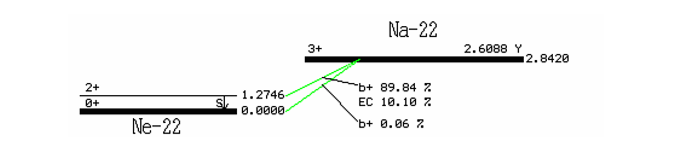
\includegraphics[scale=0.8]{Bilder/Natrium_zerfall}
	\caption[Zerfallsschema Natrium]{\small Das Zerfallsschema des verwendeten $^{22}Na$ Isotops mit allen möglichen Übergängen. Die Energien sind in MeV angegeben. Entnommen aus \cite{staatsex_szinti}}
	\label{Natrium_schema}
\end{figure}

\subsection{Cobalt}
Das hier verwendete $^{60}Co$ Isotop zerfällt über einen $\beta^-$ Zerfall in $^{60}Ni$ im angeregten Zustand. Dieser gibt seine Energie in der Regel in zwei schritten über $\gamma$ Photonen der Energien 1333 und 1173 keV ab. Das genaue Zerfallsschema ist in Abbildung \ref{Cobalt_schema} zu erkennen.
\begin{figure}
	\centering
	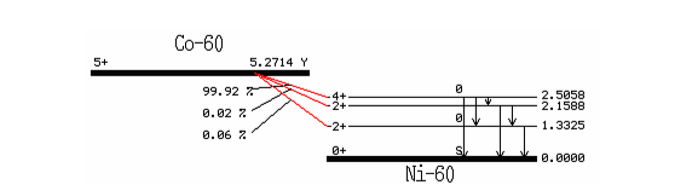
\includegraphics[scale=0.8]{Bilder/Cobalt_zerfall}
	\caption[Zerfallsschema Cobalt]{\small Das Zerfallsschema des verwendeten $^{60}Co$ Isotops mit allen möglichen Übergängen. Die Energien sind in MeV angegeben. Entnommen aus \cite{staatsex_szinti}}
	\label{Cobalt_schema}
\end{figure}

\subsection{Europium}
Das Zerfallsschema von $^{152}Eu$ ist viel Komplexer als die von Cobalt und Natrium, weshalb nur die beiden intensivsten Übergänge erwähnt werden, welche auch zur Energie Eichung verwendet wurden. Hierbei handelt es sich um die Zerfälle mit Tochterkernen $^{152}Sm$ und  $^{152}Gd$ bei welchen jeweils $\gamma$ Photonen der Energien 122 keV und 344 keV emittiert werden. Diese Vereinfachung ist in Abbildung \ref{Europium_schema}   sichtbar.
\begin{figure}
	\centering
	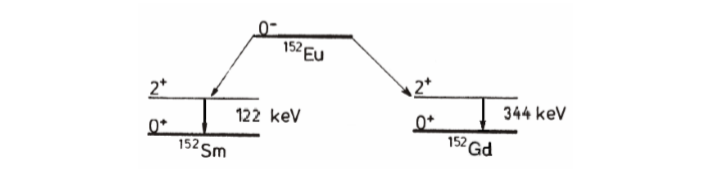
\includegraphics[scale=0.8]{Bilder/Europium_zerfall}
	\caption[Zerfallsschema Europium]{\small Das Zerfallsschema des verwendeten $^{152}Eu$ Isotops mit beiden wahrscheinlichsten Übergängen. Entnommen aus \cite{staatsex_szinti}}
	\label{Europium_schema}
\end{figure}

\subsection{Thorium}
Das hier verwendete $^{228}Th$ Isotop zerfällt über $\alpha$ und$\beta$ Zerfall unter der Emission von $\gamma$ Photonen mit  vielen Verschiedenen Energien zu $^{208}Pb$. Die Zerfallsreihe ist in Abbildung \ref{Thorium_reihe} zu sehen. Die genaue Zerfallsreihe ist zu komplex um hier genauer darauf einzugehen. Es werden in der Auswertung die Beobachteten $\gamma$ Photonen den respektive Übergängen zuzuordnen. Mehr Details zu den einzelnen Zerfällen sind in der Staatsexamensarbeit von T.Kotyk \cite{staatsex_szinti} zu finden.

\begin{figure}
	\centering
	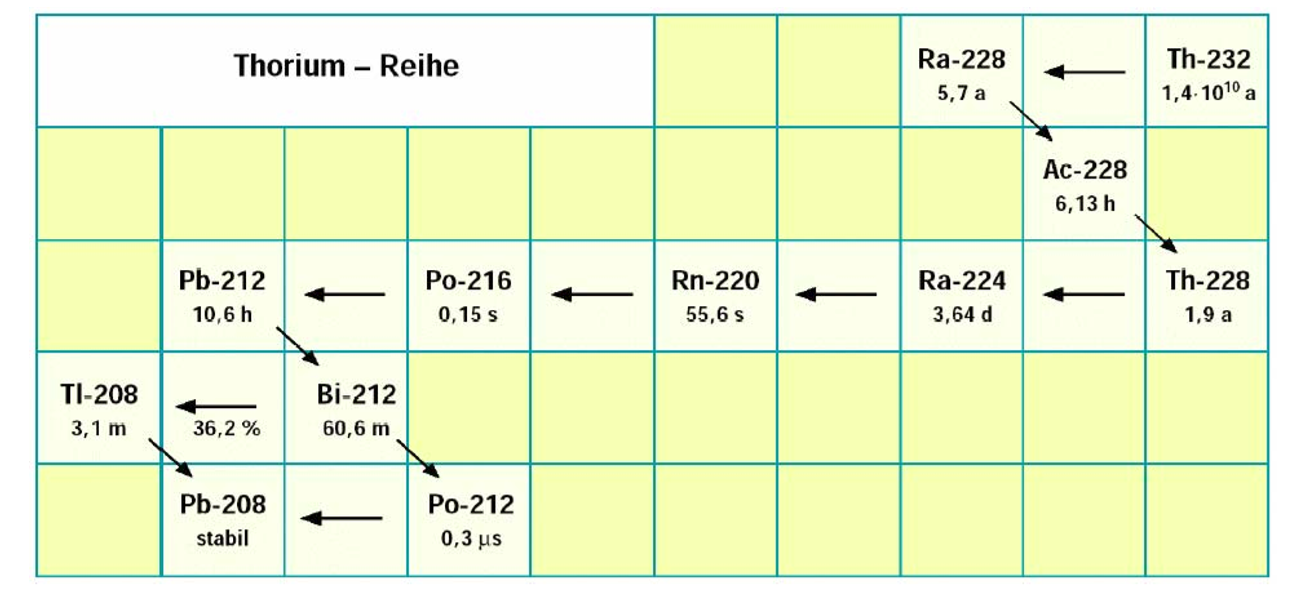
\includegraphics[scale=0.8]{Bilder/Thorium-Reihe}
	\caption[Zerfallsschema Europium]{\small Die Zerfallsreihe des verwendeten $^{228}Th$ Isotops mit allen Zwischenprodukten. Entnommen aus \cite{staatsex_szinti}}
	\label{Thorium_reihe}
\end{figure}